\documentclass{beamer}
\usepackage{sdp}

\title{Опашка}

\date{7 ноември 2017 г.}

% TODO: източник на картинката
\titlegraphic{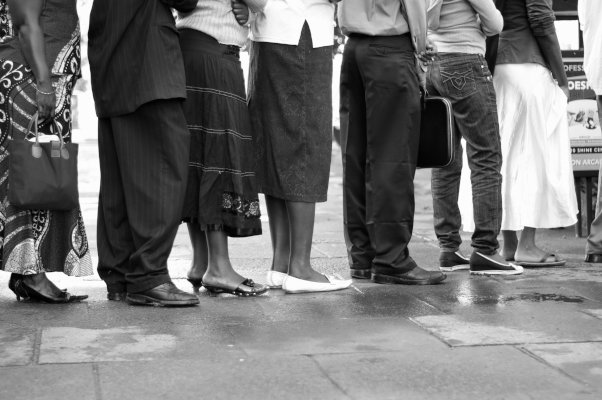
\includegraphics[height=0.35\textheight]{images/queue.jpg}}

\usetikzlibrary{decorations.pathmorphing}

\begin{document}

\begin{frame}
  \titlepage
\end{frame}

\section{АТД опашка}

\begin{frame}
  \frametitle{АТД: опашка}

  Хомогенна линейна структура с организация ``пръв влязъл --- пръв излязъл'' (FIFO)\\[1em]
  Операции:\\[0.5em]
  \begin{itemize}
  \item \lst{create()} --- създаване на празна опашка
  \item \lst{empty()} --- проверка за празнота на опашка
  \item \lst{enqueue(x)} --- включване на елемент в края на опашката
  \item \lst{dequeue()} --- изключване на елемент от началото на опашката
  \item \lst{head()} --- достъп до първия елемент
  \end{itemize}
\end{frame}

\begin{frame}
  \frametitle{АТД: опашка}

  Свойства на операциите\\[0.5em]
  \small
  \begin{itemize}
  \item \lst{create().empty()} = \lst{true}
  \item \lst{q.enqueue(x).empty()} = \lst{false}
  \item \lst{create().head()}, \lst{create().dequeue()} --- \alert{грешка}
  \item \tt{create().enqueue(x$_1$).enqueue(x$_2$)\ldots{}enqueue(x$_n$).head() = x$_1$}
  \item \tt{create().enqueue(x$_1$).enqueue(x$_2$)\ldots{}enqueue(x$_n$).dequeue() = create().enqueue(x$_2$)\ldots{}enqueue(x$_n$)}
  \end{itemize}
\end{frame}

\begin{frame}
  \frametitle{Последователно представяне}
  \newcommand{\pha}{\phantom{$a_0$}}

  % TODO: да се нарисува с TikZ
  \begin{center}
    \begin{tabular}{|*{11}{c|}}
      \hline
      \rowcolor{diagramblue}
      \alt<7-| handout:0>{$a_{n+5}$}\pha&\pha&\alt<1>{$a_0$}\pha&$a_1$&$a_2$&\ldots&$a_n$&\alt<3-| handout:0>{$a_{n+1}$}\pha&\alt<4-| handout:0>{$a_{n+2}$}\pha&\alt<5-| handout:0>{$a_{n+3}$}\pha&\alt<6-| handout:0>{$a_{n+4}$}\pha\\
      \hline
      \rowcolor{white}
      \multicolumn 1c{\onslide<7| handout:0>{\bua}}&
      \multicolumn 1c{}&
      \multicolumn 1c{\onslide<1>{\bua}}&
      \multicolumn 1c{\onslide<2-| handout:0>{\bua}}&
      \multicolumn 2c{}&
      \multicolumn 1c{\onslide<1-2| handout:1>{\bua}}&
      \multicolumn 1c{\onslide<3| handout:0>{\bua}}&
      \multicolumn 1c{\onslide<4| handout:0>{\bua}}&
      \multicolumn 1c{\onslide<5| handout:0>{\bua}}&
      \multicolumn 1c{\onslide<6| handout:0>{\bua}}\\
      \multicolumn 1c{\onslide<7| handout:0>{back}}&
      \multicolumn 1c{}&
      \multicolumn 1c{\onslide<1>{front}}&
      \multicolumn 1c{\onslide<2-| handout:0>{front}}&
      \multicolumn 2c{}&
      \multicolumn 1c{\onslide<1-2| handout:1>{back}}&
      \multicolumn 1c{\onslide<3| handout:0>{back}}&
      \multicolumn 1c{\onslide<4| handout:0>{back}}&
      \multicolumn 1c{\onslide<5| handout:0>{back}}&
      \multicolumn 1c{\onslide<6| handout:0>{back}}
    \end{tabular}
  \end{center}
  \begin{itemize}
    \item<2-> изключване на елемент (dequeue)
    \item<3-> включване на елемент (enqueue)
  \end{itemize}
\end{frame}

\begin{frame}<1-7>
  \frametitle{Свързано представяне}

  % TODO: да се нарисува с TikZ
  \begin{center}
    \scriptsize
    \begin{tabular}{cccc@{}c@{}cc}
      \onslide<1-6| handout:1>{\nextcell{a_0}}&\nextcell{a_1}&\nextcell{a_3}&\hspace{1ex}\ldots&$\nextarrow$&\alt<1,2| handout:1>{\nilcell{a_n}}{\nextcell{a_n}}&\onslide<2-| handout:0>{\nilcell{a_{n+1}}}\\
      \onslide<1-6| handout:1>{\bua}&\onslide<6-| handout:0>{\bua}&\multicolumn 3c{}&\onslide<1-3| handout:1>{\bua}&\onslide<2-| handout:0>{\bua}\\
      \only<5-6| handout:0>p\only<5| handout:0>,\only<1-5| handout:1>{front}&\onslide<6-| handout:0>{front}&\multicolumn 3c{}&\onslide<1-3| handout:1>{back}&\only<2-| handout:0>{\alt<2-3| handout:0>p{back}}
    \end{tabular}
  \end{center}
  \begin{itemize}
    \item<2-> включване на елемент (enqueue)
    \item<5-> изключване на елемент (dequeue)
  \end{itemize}
\end{frame}

\section{Задачи}

\begin{frame}
  \frametitle{Числа на Hamming}
  \newcommand{\pha}{\phantom{00}}
  \newcommand{\pho}{\phantom{0}}

  \begin{definition}
    Казваме, че $k$ е число на Hamming, ако простите делители на $k$ са сред 2, 3 и 5, т.е. $k = 2^x3^y5^z$ за $x,y,z\geq 0$.
  \end{definition}

  \textbf{Задача.} Да се изведат в нарастващ ред първите $n$ числа на Hamming.\\
  \pause
  % TODO: да се нарисува с TikZ
  \textbf{Решение:}
  \begin{center}
    \begin{tabular}{r@{\hskip 1ex}|*{11}{c|}}
      \hhline{~*{11}{-}}
      \rowcolor{diagramblue}
      \cellcolor{white}q$_2$&\alt<3-4>{\alert<4>2}\pho&\alt<4-6>{\alert<6>4}\pha&\alt<5-8>{\alert<8>6}\pha&\alt<6->8\pha&\alt<7->{10}\pha&\alt<8->{12}\pha&\pha&\pha&\pha&\pha&\pha\\
      \hhline{~*{11}{-}}
      \rowcolor{white}
      \multicolumn{12}c{}\\[0.5em]
      \hhline{~*{11}{-}}
      \rowcolor{diagramblue}
      \cellcolor{white}q$_3$&\alt<3-5>{\alert<5>3}\pho&\alt<4-8>{\alert<8>6}\pha&\alt<5->9\pha&\alt<6->{12}\pha&\alt<7->{15}\pha&\alt<8->{18}\pha&\pha&\pha&\pha&\pha&\pha\\
      \hhline{~*{11}{-}}
      \rowcolor{white}
      \multicolumn{12}c{}\\[0.5em]
      \hhline{~*{11}{-}}
      \rowcolor{diagramblue}
      \cellcolor{white}q$_5$&\alt<3-7>{\alert<7>5}\pho&\alt<4->{10}\pha&\alt<5->{15}\pha&\alt<6->{20}\pha&\alt<7->{25}\pha&\alt<8->{30}\pha&\pha&\pha&\pha&\pha&\pha\\
      \hhline{~*{11}{-}}
    \end{tabular}\\[1em]
    1%
    \onslide<5->{, 2}%
    \onslide<6->{, 3}%
    \onslide<7->{, 4}%
    \onslide<8->{, 5}%
    \onslide<9->{, 6, \ldots}
  \end{center}
\end{frame}

\begin{frame}
  \frametitle{Числа на Hamming: коректност}

  Да се докаже, че:
  \begin{enumerate}[<+->]
  \item се извеждат \textbf{всички} числа на Hamming\\
    \begin{proof}<+->
       Индукция: $2^x3^y5^z$ се извежда, понеже $2^{x-1}3^y5^z$ се извежда.
    \end{proof}
  \item се извеждат \textbf{само} числа на Hamming\\
    \begin{proof}<+->
      Ако извадим $2^x3^y5^z$, в опашките се записват $2^{x+1}3^y5^z$, $2^x3^{y+1}5^z$, $2^x3^y5^{z+1}$.
    \end{proof}
  \item числата на Hamming се извеждат във възходящ ред\\
    \begin{proof}<+->
      Да допуснем, че на края на някоя опашка добавяме по-малко число. Тогава на предна стъпка трябва да сме добавили по-малко число!
    \end{proof}
  \end{enumerate}
\end{frame}

\begin{frame}<1-9>
  \frametitle{Минимален елемент на опашка}
  \newcommand{\pha}{\phantom{8}}
  \newcommand{\sent}{\alert s}

  \textbf{Задача.} Дадена е опашка $q$. Да се изключи от $q$ най-малкият ѝ елемент, като всички останали елементи останат в опашката (не непременно в първоначалния ред).\\[1em]
  \begin{onlyenv}<handout:0>
    \pause
    \textbf{Решение:}
    % TODO: да се нарисува с TikZ
    \begin{center}
      \begin{tabular}{|*{11}{c|}}
        \hline
        \rowcolor{diagramblue}
        \alt<4->\pha5&\alt<5->\pha3&\alt<6->\pha6&\alt<7->\pha1&\alt<8->\pha2&\alt<3-8>\sent\pha&\alt<5->5\pha&\alt<6->6\pha&\alt<7->3\pha&\alt<8->2\pha&\pha\\

        \hline
      \end{tabular}
      \vspace{1em}
      \onslide<4->{min = \temporal<5-6>531}
    \end{center}
  \end{onlyenv}
\end{frame}

\begin{frame}
  \frametitle{Сортиране на опашки с пряка селекция}

\textbf{Задача.} Да се подредят елементите на опашка в нарастващ ред.
\vspace{1em}
\pause

\textbf{Решение:} Използваме нова опашка и прилагаме предната задача върху дадената опашка докато свърши, а минималните елементи поставяме в новата опашка.
\end{frame}

\begin{frame}
  \frametitle{Метод на вълната}

  \scriptsize
  % TODO: дъската да се нарисува с TiKZ
  \begin{center}
    \begin{chessboard}{10}{0.5ex}
      \hline
      \empty&\empty&\empty&\empty&\wave8&\wave7&\wave6&\wave7&\wave8&\empty&\\
      \hline
      \empty&\empty&\noway&\empty&\empty&\noway&\wave5&\wave6&\wave7&\wave8&\\
      \hline
      \empty&\empty&\noway&\empty&\empty&\noway&\wave4&\wave5&\wave6&\noway&\\
      \hline
      \empty&\empty&\empty&\empty&\noway&\wave2&\wave3&\wave4&\noway&\empty&\\
      \hline
      \empty&\empty&\empty&\noway&\wave2&\wave1&\wave2&\noway&\empty&\empty&\\
      \hline
      \noway&\empty&\empty&\noway&\wave3&\wave2&\noway&\empty&\empty&\noway&\\
      \hline
      \noway&\noway&\empty&\noway&\noway&\wave3&\noway&\noway&\empty&\empty&\\
      \hline
      \empty&\empty&\noway&\wave6&\wave5&\wave4&\noway&\empty&\empty&\noway&\\
      \hline
      \empty&\empty&\wave8&\wave7&\wave6&\wave5&\noway&\empty&\empty&\empty&\\
      \hline
      \empty&\empty&\empty&\noway&\wave7&\wave6&\wave7&\wave8&\noway&\empty&\\
      \hline
      \multicolumn 1c\empty&\multicolumn 1c\empty&\multicolumn 1c\empty&\multicolumn 1c\empty&\multicolumn 1c\empty&\multicolumn 1c\empty&\multicolumn 1c\empty&\multicolumn 1c\empty&\multicolumn 1c\empty&\multicolumn 1c\empty&
    \end{chessboard}
  \end{center}
  \only<9>{
  \begin{tikzpicture}[remember picture,overlay]
    \foreach \r in {1.5,3.2,...,12}{
      \draw[red,decorate,decoration={coil,segment length=4ex,amplitude=0.3ex},thick,xshift=21.2em,yshift=14.4em,rotate=45] (-\r em,-\r em) rectangle (\r em, \r em);
    }
  \end{tikzpicture}}
\end{frame}

\begin{frame}<handout:0>
  \frametitle{Ход на коня --- най-кратък път}
  \setboardfontsize{16pt}

  \def\arraystretch{0}
  % TODO: да се нарисува с TikZ
  \begin{center}
    \begin{tabular}{|*{10}{@{}c@{}|}@{}c@{}}
      \hline
      \bkn1&\bkn4&\bkn3&\bkn4&\bkn3&\bkn4&\bkn5&\ws  &\bkn5&\ws  &\\
      \hline
      \bkn4&\bkn5&\bkn2&\bkn5&\bkn4&\bkn5&\bkn4&\bkn5&\ws  &\ws  &\\
      \hline
      \bkn3&\bkn2&\bkn5&\bkn4&\bkn3&\bkn4&\bkn5&\ws  &\bkn5&\ws  &\\
      \hline
      \bkn4&\bkn5&\bkn4&\bkn3&\bkn4&\bkn5&\bkn4&\bkn5&\ws  &\ws  &\\
      \hline
      \bkn3&\bkn4&\bkn3&\bkn4&\bkn5&\bkn4&\bkn5&\ws  &\bkn5&\ws  &\\
      \hline
      \bkn4&\bkn5&\bkn4&\bkn5&\bkn4&\bkn5&\ws  &\bkn5&\ws  &\ws  &\\
      \hline
      \bkn5&\bkn4&\bkn5&\bkn4&\bkn5&\ws  &\bkn5&\ws  &\ws  &\ws  &\\
      \hline
      \ws  &\bkn5&\ws  &\bkn5&\ws  &\bkn5&\ws  &\ws  &\ws  &\ws  &\\
      \hline
      \bkn5&\ws  &\bkn5&\ws  &\bkn5&\ws  &\ws  &\ws  &\ws  &\ws  &\\
      \hline
      \ws  &\ws  &\ws  &\ws  &\ws  &\ws  &\ws  &\ws  &\ws  &\ws  &\\
      \hline
    \end{tabular}
  \end{center}
\end{frame}

\section{STL}

\begin{frame}
  \frametitle{\lst{stl::queue<T>}}

  \begin{itemize}
  \item \lst{queue()} --- създаване на празна опашка
  \item \lst{empty()} --- проверка за празнота на опашка
  \item \lst{push(x)} --- включване на първи елемент в опашката
  \item \lst{pop()} --- изключване на последен елемент от опашката
  \item \lst{front()} --- първи елемент в опашката
  \item \lst{back()} --- последен елемент в опашката
  \item \lst{size()} --- дължина на опашката
  \item \lst{==,!=,<,>,<=,>=} --- лексикорафско сравнение на две опашки
  \end{itemize}
\end{frame}

\end{document}
